\bluepage{Per-fragment operations / Per fragment operace}

\begin{frame}[fragile]\frametitle{Per fragment operace}\scriptsize
  \begin{itemize}
  \item Per-fragment operations are applied on fragments after fragment shader.
  \item The most important operation is visibility determination using depth test.
  \item Visibility in OpenGL is computed using depth buffer.
  \item There are other tests, stencil, scissor tests, ...
  \item Other per-fragment operation is blending used for transparency.
  \end{itemize}
  \begin{itemize}
  \item Po fragment shaderu jsou na fragmenty aplikovány Per fragment operace.
  \item Nejzákladnější operací je řešení viditelnosti pomocí depth testu.
  \item Viditelnost se v OpenGL řeší pomocí depth bufferu (paměť hloubky).
  \item Další testy jsou stencil test a scissor test.
  \item Mezi jiné operace patří blending, který se využívá pro průhledné objekty.
  \end{itemize}
\end{frame}


\begin{frame}[fragile]\frametitle{Depth Test a Depth Buffer}\scriptsize
  \begin{itemize}
  \item Depth test solves visiblity using depth buffer (on the fragment level).
  \item Different modes of comparison of depths.
  \item Depth precision is not infinite (usually 24 bits).
  \item The common problem is depth fight (z-fight).
  \item Early depth test - the depth test can be executed before fragment shader.
  \item Early depth test can be executed, if the fragment shader does not modify the depth.
  \item Early depth test can dramatically increase the performace.
  \end{itemize}
  \begin{itemize}
  \item Depth test řeší viditelnost pomocí Depth Bufferu a to na úrovni fragmentů.
  \item Různé způsoby nastavení.
  \item Přesnost depth bufferu není nekonečná (většinou 24 bitů).
  \item Častý problem depth bufferu je jev známý jako depth fight.
  \item Brzký depth test - depth test může předběhnout vykonávání fragment shaderu.
  \item Brzký depth test se provádí tehdy, pokud se ve fragment shaderu nemodifikuje hloubka fragmetu.
  \item Brzký depth test může značně urychlit kreslení.
  \end{itemize}
  {\scriptsize
\begin{minted}[bgcolor=bg]{packages/c_cpp.py:CppLexer -x}
glEnable(GL_DEPTH_TEST);//enable depth test
glDepthFunc(GL_LEQUAL);//set the comparison operator
glDepthMask(GL_TRUE);//enable writes into depth buffer
  \end{minted}
  }
\end{frame}

\begin{frame}[fragile]\frametitle{Blending - transparent object}\scriptsize
  \begin{itemize}
  \item Blending provides the ability to mix fragment colors with framebuffer colors.
  \item The main goal of blending is to enable transparency.
  \item Blending is driven by blend operation, source and destination factors.
  \item Blending operation can be addition, subtraction, min, max, ...
  \item The source factor comes from fragment values (alpha, color, 1-alpha, ...)
  \item The destination factor comes from framebuffer (alpha, color, 1-alpha, ...)
  \item In order to properly compute transparency, transparent triangles must be sorted.
  \end{itemize}
  \begin{itemize}
  \item Blending umožňuje kombinovat novou barvu s již zapsanou barvou ve framebufferu.
  \item Blending je řízen pomocí blendovací operace, source a destination faktorů.
  \item Blendovací operace jsou sčítání, odčítání, min, max, ...
  \item Source faktor se aplikuje na barvu fragmentu.
  \item Destination faktor se aplikuje na barvu již uloženou ve framebufferu.
  \item Nutnost kreslit ve správném pořadí.
  \end{itemize}
  \begin{figure}[h]
  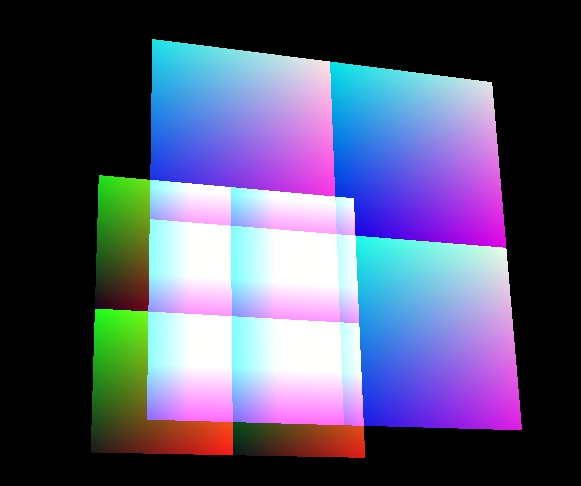
\includegraphics[width=3cm,keepaspectratio]{pics/pfo/blending.jpg}
  \end{figure}
  {\scriptsize
\begin{minted}[bgcolor=bg]{packages/c_cpp.py:CppLexer -x}
glEnable(GL_BLEND);//enable blending
glBlendEquation(GL_FUNC_ADD);//binding operation
glBlendFunc(GL_SRC_ALPHA,GL_ONE_MINUS_SRC_ALPHA);//source, destinaion factors.
  \end{minted}
  }
\end{frame}

